\subsection{Performance}\label{performance}

Although the performance and efficiency of a distributed application mostly depends on the employed programming models and patterns and their suitability for the underlying distributed infrastructure (a choice that can only be made by the developer), SAGA exposes certain performance characteristics and pitfalls that should be taken into consideration when developing distributed applications. Besides a negligible overhead generated by the Engine and its dynamic adaptor loading and selection mechanism (\ref{perf_engine}) SAGA's performance is governed by two major factors: The performance of the middleware adaptor implementations (\ref{perf_adaptors}) and the usage of SAGA's asynchronous interface and task-based operations (\ref{perf_async}). We carried out several benchmarks to pinpoint SAGA’s performance in a production-level environment.   We used an unmodified version of the current SAGA release (1.2.1) on various TeraGrid resources over an extended period of time (to filter out system noise) and where appropriate compared the results to the native middleware tools. In the following, we present our results and discuss their implications for application developers. 

\begin{figure}[!ht]
  \begin{center}
      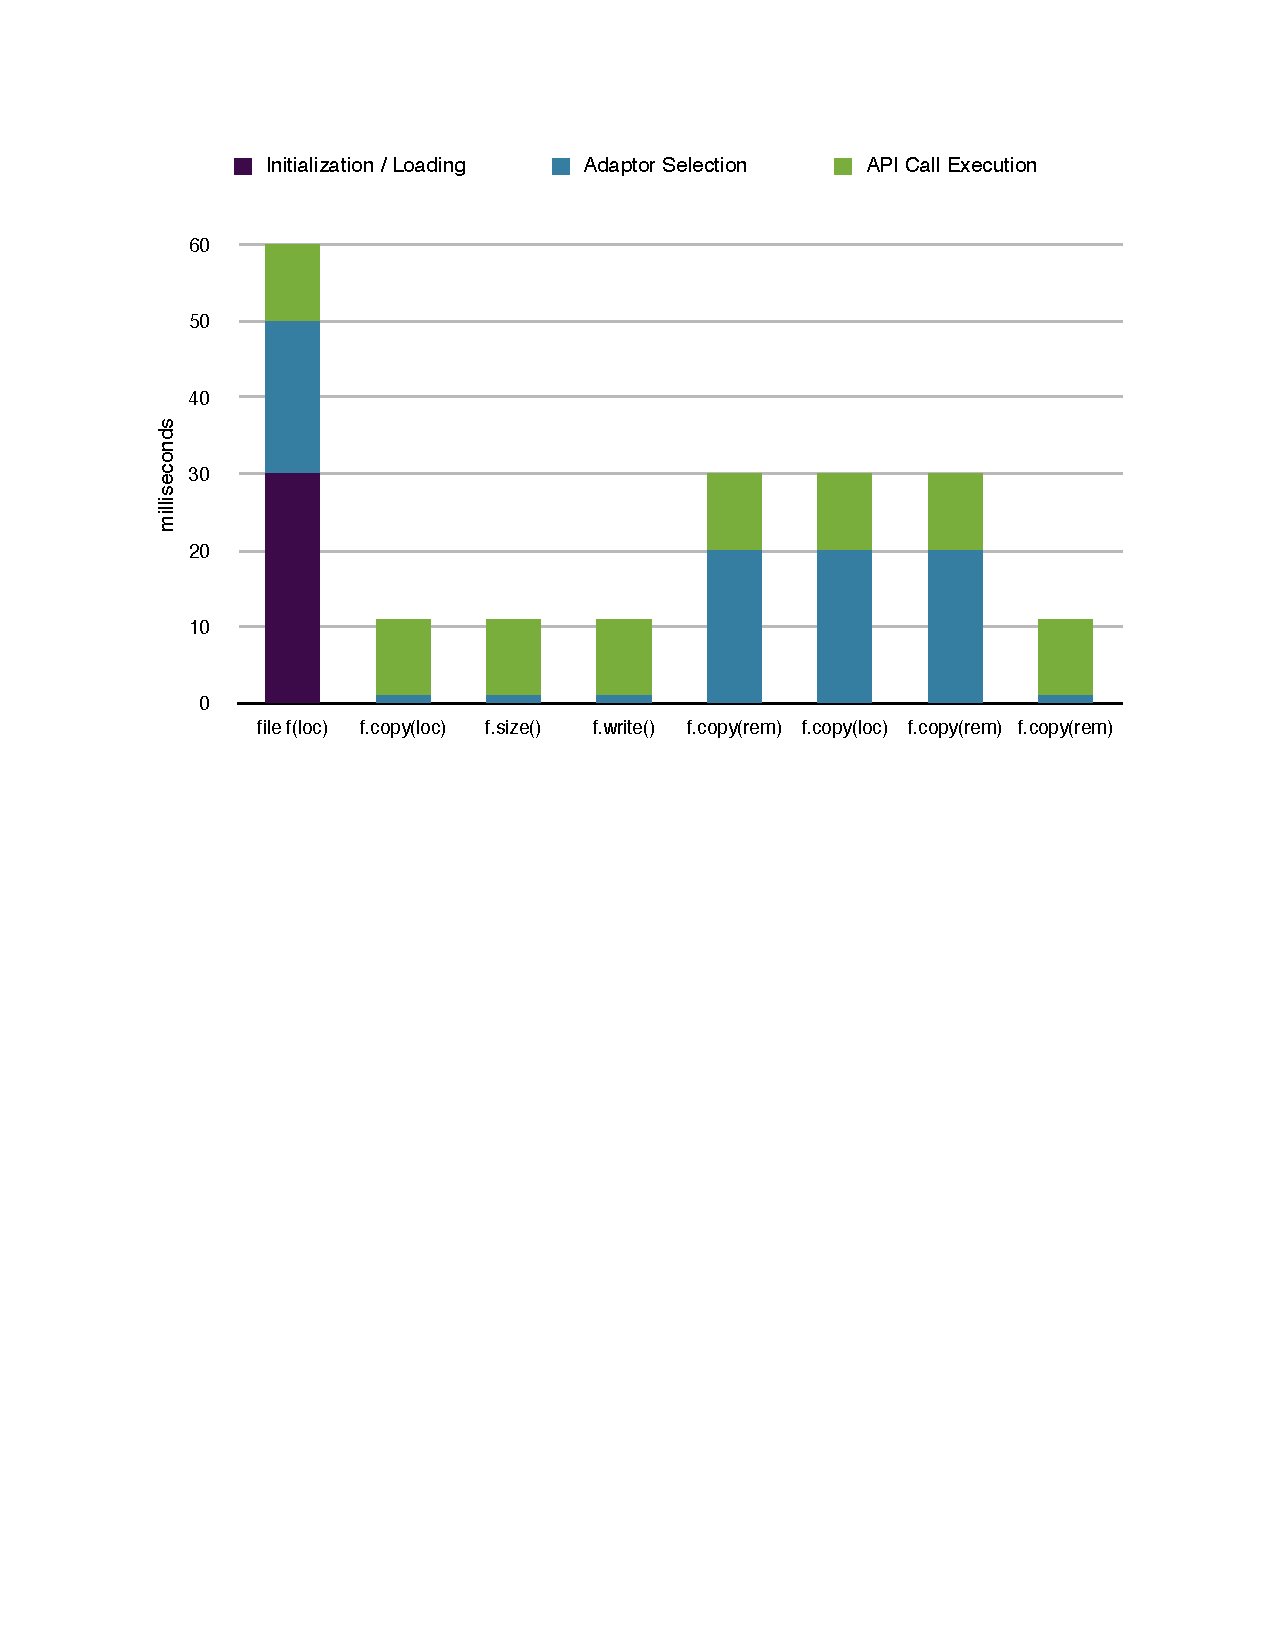
\includegraphics[width=1\textwidth]{../figures/perf_overhead.pdf}
  \end{center}
 \up\up\up\up\up
  \caption{\small Execution times for several SAGA file operations. The first API invocation triggers the initialization and adaptor loading process. The three subsequent calls have virtually no overhead thanks to adaptor priorization. Call 5 to 7 iterate between two different adaptors to execute local (loc) and remote (rem) file copy which causes some adaptor selection overhead.}
 \label{fig_perf_overhead}
\end{figure}

\subsubsection{Engine Performance}\label{perf_engine}
The selection of suitable adaptors to execute an API call at runtime is one of the key features of our C++ SAGA implementation. Naturally, it comes with a certain overhead since it involves several logical steps as depicted in Figure (1). On startup, the Engine parses its configuration file (saga.ini), loads all configured middleware adaptors (dynamic libraries) and registers their capabilities in an internal data structure. The overhead generated by this step varies with the number of configured adaptors but lies generally in the range of 30 milliseconds on an average system. 
If an API method is to be executed, the Adaptor Selector searches the internal adaptor registry for all Adaptors that could potentially execute the API call and tests them one by one.

Our experience with SAGA-based application shows that there’s a high probability that the same adaptor will be selected for many subsequent API calls. In fact, most applications use only one specific middleware Adaptor throughout their entire lifetime. The Engine addresses this by putting the adaptor that executed the last API call in the first position of the registry. This completely eliminates potential adaptor selection overhead for subsequent calls as depicted in Figure \ref{fig_perf_overhead}. But even if this mechanism doesn't kick in due to frequent adaptor changes, the overhead exposed by the adaptor selection is in the order of 20 milliseconds which lies several orders of magnitudes below the typical latencies of a distributed application.


\subsubsection{Adaptor Performance}\label{perf_adaptors}

\begin{figure}[!ht]
  \begin{center}
      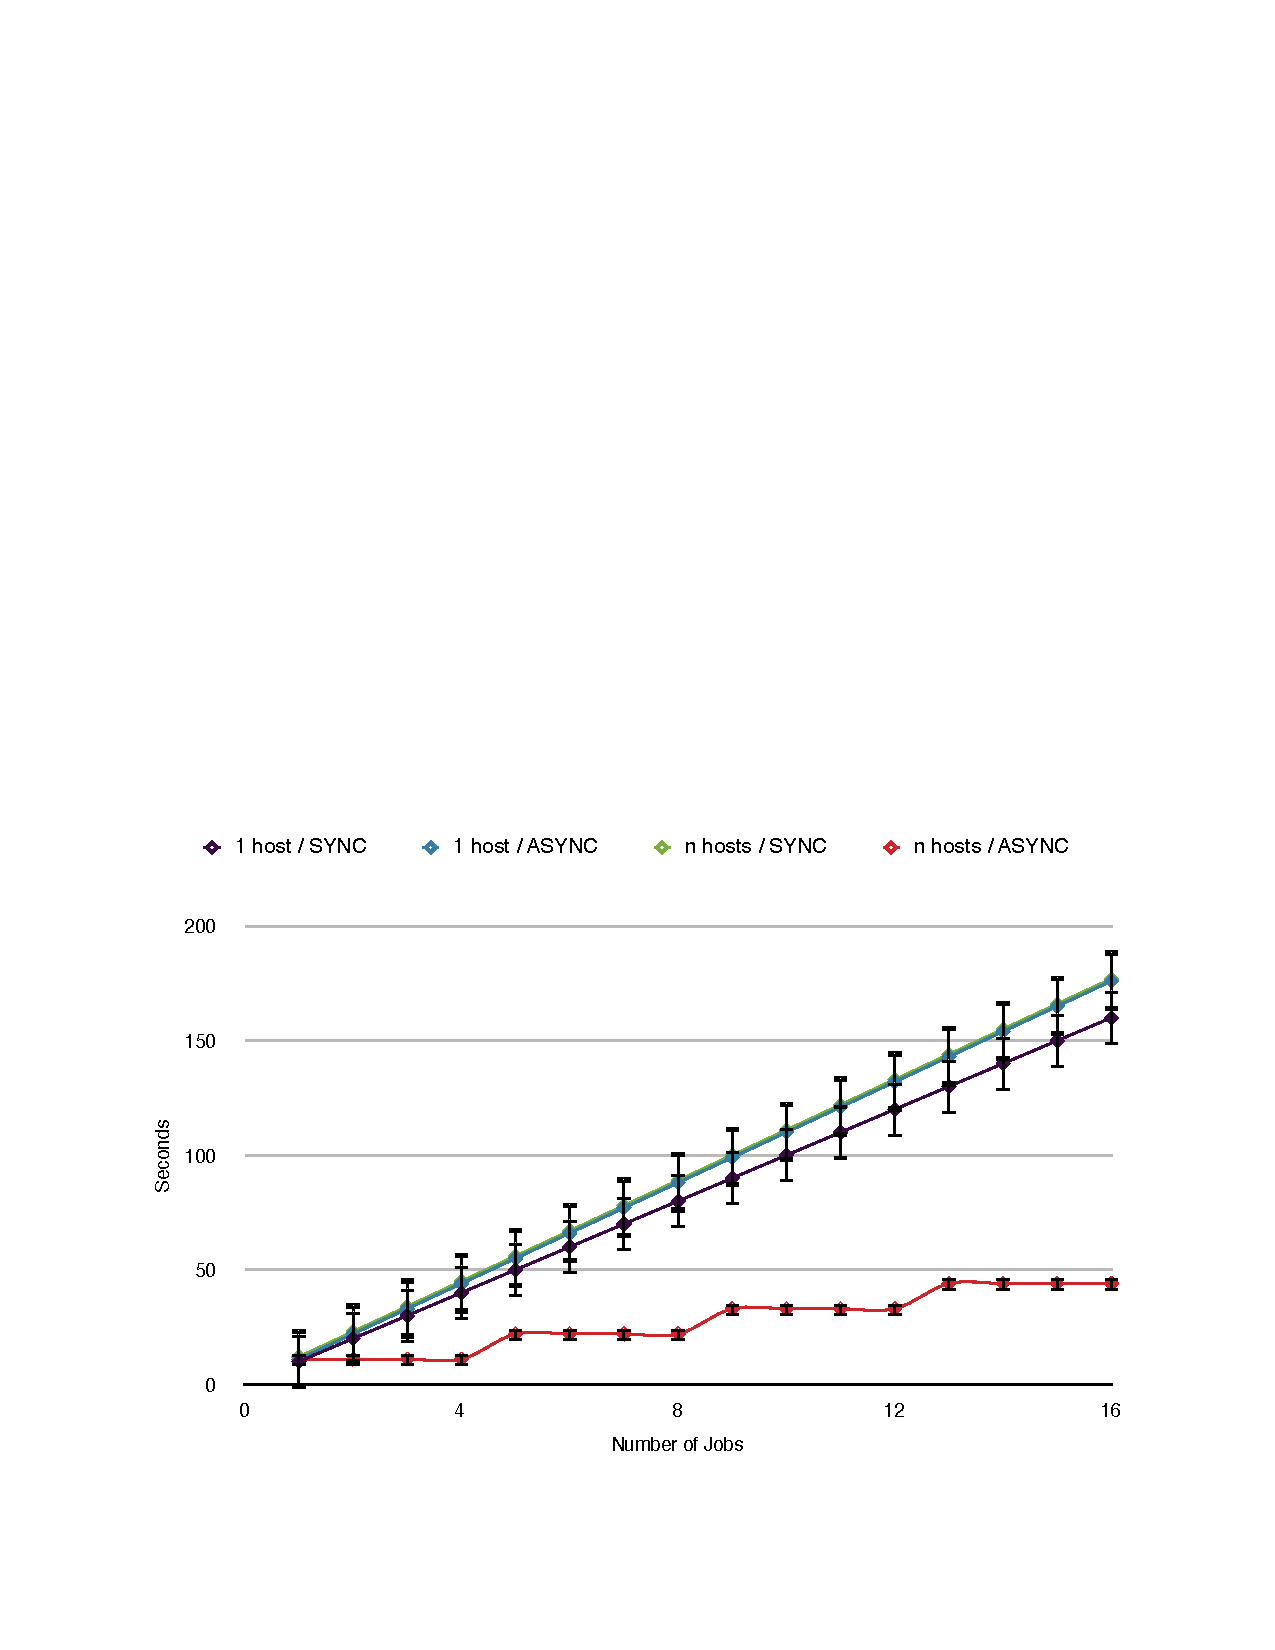
\includegraphics[width=1\textwidth]{../figures/perf_async_1.pdf}
  \end{center}
 \up\up\up\up\up
  \caption{\small Comparison of sync/async execution times for SAGA job submission operations (using the Globus GRAM adaptor) in different scenarios. The linear increase of the execution time submitting \texttt{n} jobs to 1 host (purple) and to \texttt{n} hosts (green) synchronously doesn't surprise. The linear increase of the execution time submitting \texttt{n} jobs to 1 host (blue) asynchronously can be counterintuitive if the underlying system infrastructure is not properly understood. In this scenario, the resource manager on the target machines accepts only one job at a time. That is the reason why only submitting \texttt{n} jobs to \texttt{n} hosts (red) asynchronously scales as expected.}
 \label{fig_perf_async}
\end{figure}

\subsubsection{Asynchronous Performance}\label{perf_async}
The asynchronous interface~\cite{saga-spec} is one of the central concepts of the SAGA API design and one of the fundamental requirements for effective latency hiding in distirbuted applications It provides an asynchronous execution model for all available API calls and thread-based runtime support for transparent execution: if a middleware adaptors doesn't implement the asynchronous interface directly, the SAGA engine simply wraps all adaptor method calls in a thread which allows for concurrent API call execution.
Naturally, threaded execution comes with a certain overhead for thread creation and management. We benchmarked a series of single API calls executed synchronously and asynchronously. The measured overhead exposed by the asynchronous interface is about XX milliseconds, which is of no consequence, considered that a typical distributed operation carried out trough SAGA (e.g. file copy, job submission) is usually in the order of seconds or even minutes. 

Although easy to use, the async interface requires a good understanding of the underlying infrastructure in order to use it \textit{efficiently}. Naively one could think that a system with \texttt{N} cores can execute \texttt{N} threads at the same time; hence, executing \texttt{N} SAGA calls concurrently will give us a speedup by the factor \texttt{N}. That this is not necessarily the case is shown in Figures \ref{fig_perf_async} and \ref{fig_perf_todo}. EXPLAIN WHY.


